\documentclass[tikz,border=8pt]{standalone}
% Shared look for every TikZ diagram. Load with \input{../../tools/tikz-style.tex}
\usepackage[sfdefault]{roboto}
\usetikzlibrary{arrows.meta, positioning, shapes.geometric, calc, fit, backgrounds}
\definecolor{cblue}{HTML}{4C78A8}
\definecolor{corange}{HTML}{F58518}
\definecolor{cgreen}{HTML}{54A24B}
\definecolor{cred}{HTML}{E45756}
\definecolor{cpurple}{HTML}{B279A2}
\definecolor{cgrey}{HTML}{6B6B6B}
\tikzset{
  every picture/.style={font=\sffamily, line width=1.2pt},
  box/.style={draw=#1, fill=#1!12, rounded corners=4pt, align=center, inner sep=7pt, minimum height=1.1cm},
  box/.default=cgrey,
  arrow/.style={-{Stealth[length=3mm]}, draw=cgrey, line width=1.4pt},
  title/.style={font=\sffamily\bfseries\Large},
  note/.style={font=\sffamily\small, text=cgrey, align=center},
}
\AtBeginDocument{\hyphenpenalty=10000 \exhyphenpenalty=10000}

% Grubler's formula on two planar mechanisms. Left: the 2R arm on the robot: ground plus 2 links (N = 3), 2 revolute
% joints (J = 2): 3(3 - 1 - 2) + 2 = 2. Right: a closed loop: ground plus 3 links (N = 4), 4 revolute joints
% (J = 4): 3(4 - 1 - 4) + 4 = 1. Revolute joints are open circles.
\begin{document}
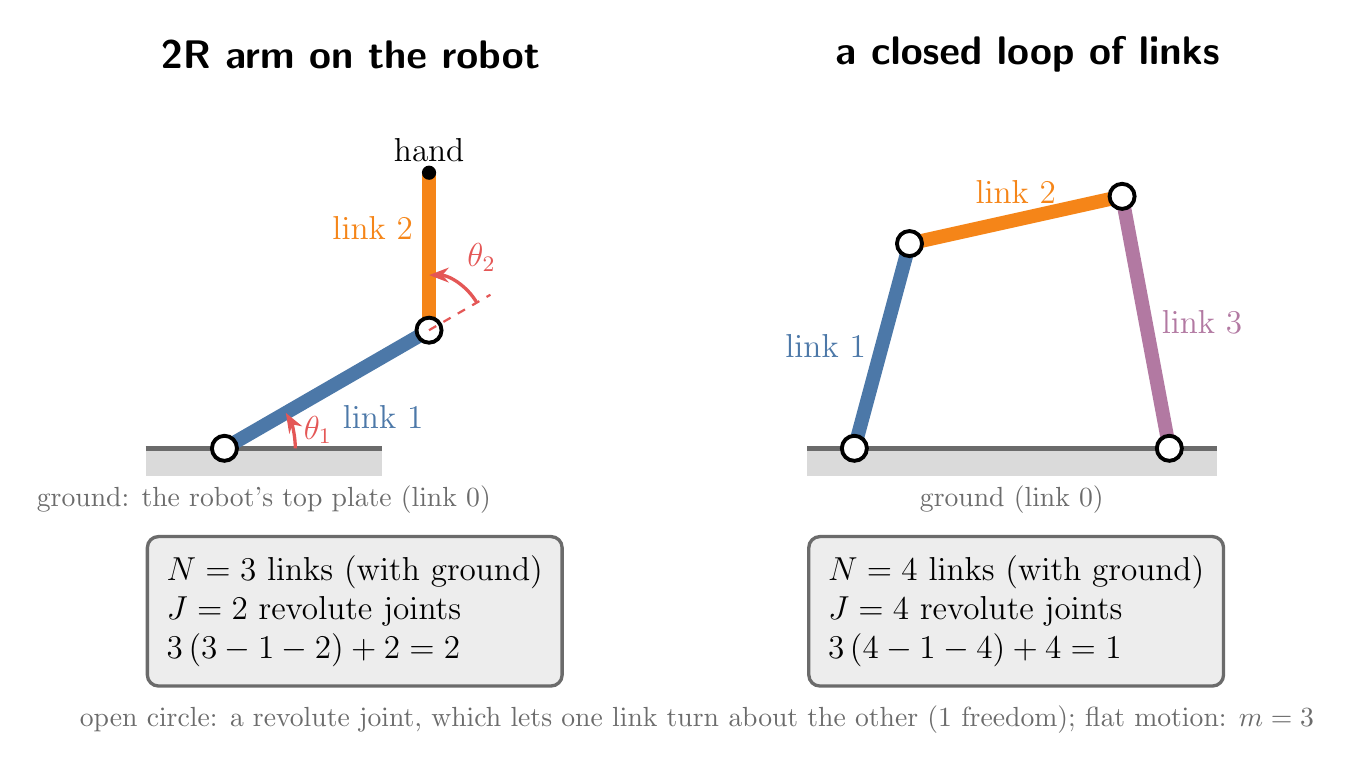
\begin{tikzpicture}[every node/.append style={font=\large}, joint/.style={circle, draw=black, fill=white, line width=1.4pt, inner sep=3.2pt}]
  % ---- the 2R arm
  \node[title] at (2.0,5.0) {2R arm on the robot};
  \fill[cgrey!25] (-0.6,0) rectangle (2.4,-0.35);
  \draw[cgrey, line width=2pt] (-0.6,0) -- (2.4,0);
  \node[cgrey, font=\normalsize] at (0.9,-0.65) {ground: the robot's top plate (link 0)};
  \coordinate (S) at (0.4,0);
  \coordinate (E) at ($(S)+(30:3.0)$);
  \coordinate (Hd) at ($(E)+(90:2.0)$);
  \draw[cblue, line width=5pt] (S) -- (E) node[midway, below right, font=\large] {link 1};
  \draw[corange, line width=5pt] (E) -- (Hd) node[pos=0.65, left, font=\large] {link 2};
  \node[joint] at (S) {};
  \node[joint] at (E) {};
  \fill[black] (Hd) circle (0.09);
  \node[above] at (Hd) {hand};
  \draw[cred, line width=1.2pt, -{Stealth[length=2.5mm]}] ($(S)+(0.9,0)$) arc (0:30:0.9) node[midway, right, text=cred] {$\theta_1$};
  \draw[cred, dashed, line width=0.8pt] (E) -- ($(E)+(30:0.9)$);
  \draw[cred, line width=1.2pt, -{Stealth[length=2.5mm]}] ($(E)+(30:0.7)$) arc (30:90:0.7) node[midway, above right, text=cred] {$\theta_2$};
  \node[box=cgrey, align=left, anchor=north west, font=\large] at (-0.6,-1.1) {$N = 3$ links (with ground)\\ $J = 2$ revolute joints\\ $3\,(3 - 1 - 2) + 2 = 2$};

  % ---- the closed loop
  \begin{scope}[xshift=8.4cm]
  \node[title] at (2.2,5.0) {a closed loop of links};
  \fill[cgrey!25] (-0.6,0) rectangle (4.6,-0.35);
  \draw[cgrey, line width=2pt] (-0.6,0) -- (4.6,0);
  \node[cgrey, font=\normalsize] at (2.0,-0.65) {ground (link 0)};
  \coordinate (P0) at (0,0); \coordinate (P3) at (4,0);
  \coordinate (P1) at (0.7,2.6); \coordinate (P2) at (3.4,3.2);
  \draw[cblue, line width=5pt] (P0) -- (P1) node[midway, left] {link 1};
  \draw[corange, line width=5pt] (P1) -- (P2) node[midway, above] {link 2};
  \draw[cpurple, line width=5pt] (P2) -- (P3) node[midway, right] {link 3};
  \foreach \p in {P0,P1,P2,P3} \node[joint] at (\p) {};
  \node[box=cgrey, align=left, anchor=north west, font=\large] at (-0.6,-1.1) {$N = 4$ links (with ground)\\ $J = 4$ revolute joints\\ $3\,(4 - 1 - 4) + 4 = 1$};
  \end{scope}
  \node[note, font=\normalsize] at (6.4,-3.45) {open circle: a revolute joint, which lets one link turn about the other (1 freedom); flat motion: $m = 3$};
\end{tikzpicture}
\end{document}
